
\section{Minimum Spanning Trees}\label{greedy: sec: MST}\doHeader{Minimum Spanning Trees}

In this section, we first consider an iterative algorithm
that is designed to maintain the greedy invariant:

\medskip 
\centerline{\textsf{greedy invariant}: the current (partial) solution can be extended to some correct (full) solution.}
\medskip 

This invariant implies correctness.
We then consider how the algorithm can instead be viewed as
making one greedy choice, then recursing.
This view also yields other algorithms.

\paragraph{Problem Definition.}

The \prob{Minimum Spanning Tree} (MST) problem is defined as follows:

\begin{mylist}
\item[\bf input:] A connected, undirected (!), edge-weighted graph $G=(V,E)$.
\item[\bf output:] A minimum-weight \emph{spanning tree} of $G$.
  (A spanning tree is a tree $T$ in $G$ whose vertex set includes all the vertices.
  The weight of $T$ is the sum of its edges' weights,
  so $\weight T = \sum_{e\in T} \weight e$.)
  We represent $T$ as the set of its edges.
\end{mylist}
Intuitively, the problem is to connect all vertices in the graph at minimum cost.

\emph{[Consider some examples to get intuition.]}
% Exercise: Give an example where a shortest-path tree
% has much larger total weight than a minimum-spanning tree.
% Give an example where the path between two vertices in a minimum-spanning tree
% is much longer than their shortest-path distance.]}

\subsection{Iterative approach (Prim's algoritm)}\label{greedy: sec: prims}
We have in mind that the greedy algorithm will build a tree edge by edge.
To build intuition,
let's start by considering candidate rules for the first step.

Suppose you know that, for some vertex $v$, there are three edges out of $v$,
weighted as follows:

\tikzset{% >= latex,
  vertex/.style ={circle, draw=black, minimum width = 20pt, inner sep=0pt},
  subtree/.style={
    draw,dotted,shape border uses incircle, yshift=30pt, % fill=lightgray,
    isosceles triangle,shape border rotate=90, % yshift=-1.45cm
    minimum height=40pt,
    minimum width=60pt,
    isosceles triangle stretches,
  }
}

\begin{center}
\begin{tikzpicture}
  \node[vertex] (v) {$a$}; 
  \node[vertex] (w1) [below =of v, xshift=-1.5cm]{$b$}; 
  \node[vertex] (w2) [below =of v, xshift=0cm]{$c$}; 
  \node[vertex] (w3) [below =of v, xshift=1.5cm]{$d$}; 
  \node[subtree] (t1) [below =of w1]{}; 
  \node[subtree] (t2) [below =of w2]{}; 
  \node[subtree] (t3) [below =of w3]{}; 

  % (r) edge[treeEdge, dotted] (u)
  \draw (v) -- (w1) node[midway, left] {\footnotesize 3}; 
  \draw (v) -- (w2) node[midway, left] {\footnotesize 1}; 
  \draw (v) -- (w3) node[midway, left] {\footnotesize 4}; 
\end{tikzpicture}
\end{center}

You don't know anything else about the rest of the graph.
Is there an edge among these three that you know \emph{must} in at least one MST?

It seems plausible that the cheapest edge $(a, c)$ should be.  Let's conjecture as follows:

\newcommand{\PRIMRULE}{
  Let $G=(V,E)$ be any connected, edge-weighted graph.
  Let $u'$ be any vertex in $V$.
  Among edges leaving $u'$, let $(u', w')$ be one of minimum weight.
  Then there exists an MST of $G$ that contains $(u', w')$.
}

\begin{conjecture}\label{greedy: conj: Prim} \PRIMRULE
 \end{conjecture}

If the conjecture is true, then, in the example, $(a, c)$ must be in some MST.

Can we prove the conjecture in general?
Consider any graph $G$ and edge $(u', w')$, as in the conjecture.
Consider any minimum-spanning tree $T^*$ for $G$.
What can we say about $T^*$?
In the case that $(u', w')$ happens to be in $T^*$, then the conjecture holds for $G$.
But what about the case where $(u', w')$ is not in $T^*$?
Can we use an exchange argument,
somehow modifying $T^*$ to add $(u', w')$ 
so as to obtain an MST that does contain $(u',w')$?

Because $T^*$ is connected and every vertex is in $T^*$,
% [review 2026-09-27] fix: vertex was written $v'$ but the discussion is about $u'$ (see the next sentence); changed to $u'$
there has to be at least one edge in $T^*$ into $u'$.
Let $(u', w^*)$ be an edge in $T^*$ incident to $u'$.
What if we construct $T'$ from $T^*$ by removing $(u', w^*)$ and replacing it by $(u', w')$?
That is, let $T' = \{(u', w')\} \cup T^* \setminus \{(u', w^*)\}$.

Then the weight of $T'$ is no larger than the weight of $T^*$,
because
\[ \weight {T'} = \weight {T^*} + \weight {u', w'} - \weight {u', w^*} \le \weight {T^*}. \]
(Here we are using that $(u', w')$ has minimum weight among edges leaving $u'$,
so $\weight {u', w'} \le \weight {u', w^*}$.)
And $T'$ does contain $(u', w')$.
Can we conclude that $T'$ is a minimum-spanning tree that contains $(u', w')$, as desired?

No!  Our reasoning has a gap that hides an error.
As we've defined $T'$, it might not be a spanning tree!
Consider the 5-vertex graph $G$ shown on the left below.
Consider the minimum spanning tree $T^*$ formed by the four solid edges in the graph on the left.

\begin{center}
\begin{tikzpicture}[scale=0.5]
  \node[vertex] (v) {$a$}; 
  \node [right =of v] {$T^*$ \Large $~\longrightarrow$}; 
  \node[vertex] (w1) [below =of v, xshift=-1.5cm]{$b$}; 
  \node[vertex] (w2) [below =of v, xshift=0cm]{$c$}; 
  \node[vertex] (w3) [below =of v, xshift=1.5cm]{$d$}; 
  \node[vertex] (x1) [below =of w3, xshift=-1.5cm]{$f$}; 

  % (r) edge[treeEdge, dotted] (u)
  \draw[ultra thick] (v) -- (w1) node[midway, left] {\footnotesize 3}; 
  \draw[dashed] (v) -- (w2) node[midway, left] {\footnotesize 1}; 
  \draw (v) -- (w3) node[midway, left] {\footnotesize 1}; 
  \draw (w3) -- (x1) node[midway, left] {\footnotesize 0}; 
  \draw (w2) -- (x1) node[midway, left] {\footnotesize 0}; 
  \draw[dotted] (w1) -- (x1) node[midway, left] {\footnotesize 4}; 
\end{tikzpicture}
\begin{tikzpicture}[scale=0.5]
  \node[vertex] (v) {$a$}; 
  \node [left =of v] {$T'$}; 
  \node[vertex] (w1) [below =of v, xshift=-1.5cm]{$b$}; 
  \node[vertex] (w2) [below =of v, xshift=0cm]{$c$}; 
  \node[vertex] (w3) [below =of v, xshift=1.5cm]{$d$}; 
  \node[vertex] (x1) [below =of w3, xshift=-1.5cm]{$f$}; 

  % (r) edge[treeEdge, dotted] (u)
  \draw[dashed] (v) -- (w1) node[midway, left] {\footnotesize 3}; 
  \draw[ultra thick] (v) -- (w2) node[midway, left] {\footnotesize 1}; 
  \draw (v) -- (w3) node[midway, left] {\footnotesize 1}; 
  \draw (w3) -- (x1) node[midway, left] {\footnotesize 0}; 
  \draw (w2) -- (x1) node[midway, left] {\footnotesize 0}; 
  \draw[dotted] (w1) -- (x1) node[midway, left] {\footnotesize 4}; 
\end{tikzpicture}
\end{center}

The edge $(a, c)$ is a minimum-weight edge among edges out of $a$, but $(a,c)$ is not in $T^*$.
The proposed reasoning suggests that we obtain $T'$ from $T^*$
by adding $(a, c)$ and removing any other edge out of $a$.
So we could, say, remove edge $(a, b)$.
% [review 2026-09-27] fix: the notation above uses $u'$ (not $v$) for the vertex; "$a$ is $v$" changed to "$a$ is $u'$"
(In the notation above, $a$ is $u'$, $c$ is $w'$, and $b$ is $w^*$.)
So $T'=\{(a,c)\}\cup T^* \setminus \{(a, b)\}$.
This is the set of solid edges shown to the right above.
But this set $T'$ is not a spanning tree,
so our proposed reasoning is flawed!

We need to study more carefully what kinds of edge exchanges we can do with spanning trees.
The next observation describes the main kind of edge exchange that we'll use.

\begin{observation}\label{greedy: exchange}
  Let $T^*$ be any spanning tree of $G$.
  Let $(u',w')$ be any edge not in $T^*$,
  and let $(x, y)$ be any edge that lies on the path in $T^*$ between $u'$ and $w'$.
  Then adding $(u', w')$ to $T^*$ and removing $(x, y)$
  % [review 2026-09-27] fix: the observation's tree is $T^*$, not $T$
  gives a spanning tree $T'=\{(u', w')\}\cup T^* \setminus \{(x, y)\}$.
\end{observation}

\begin{center}
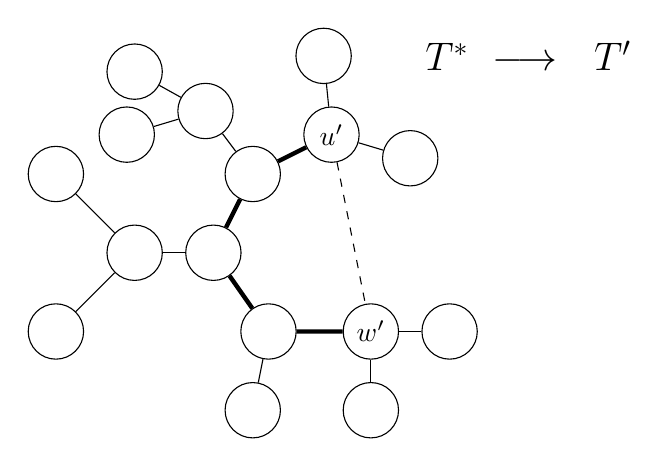
\begin{tikzpicture}
  \node[vertex] (v) at (3, 3.5) {$u'$}; 
  \node[vertex] (c1) at (2, 3) {}; 
  \node[vertex] (c2) at (1.5, 2) {}; 
  \node[vertex] (c3) at (2.2, 1) {}; 
  \node[vertex] (wp) at (3.5, 1) {$w'$}; 
  \node[vertex] (v1) at (2.9, 4.5) {};
  \node[vertex] (v2) at (4, 3.2) {}; 
  \node[vertex] (c11) at (1.4, 3.8) {}; 
  \node[vertex] (c111) at (0.5, 4.3) {}; 
  \node[vertex] (c112) at (0.4, 3.5) {}; 
  \node[vertex] (c21) at (0.5, 2) {}; 
  \node[vertex] (c211) at (-0.5, 3) {}; 
  \node[vertex] (c212) at (-0.5, 1) {}; 
  \node[vertex] (c31) at (2, 0) {}; 
  \node[vertex] (w1) at (4.5, 1) {}; 
  \node[vertex] (w2) at (3.5, 0) {}; 
  \node at (5.5, 4.5) {\Large $T^*~\longrightarrow~~T'$}; 
  % (r) edge[treeEdge, dotted] (u)
  \draw[dashed] (v) -- (wp); 
  \draw[ultra thick] (v) -- (c1) -- (c2) -- (c3) -- (wp); 
  \draw (v1) -- (v) -- (v2); 
  \draw (c1) -- (c11); 
  \draw (c2) -- (c21); 
  \draw (c3) -- (c31); 
  \draw (c111) -- (c11) -- (c112); 
  \draw (c211) -- (c21) -- (c212); 
  \draw (w1) -- (wp) -- (w2); 
\end{tikzpicture}
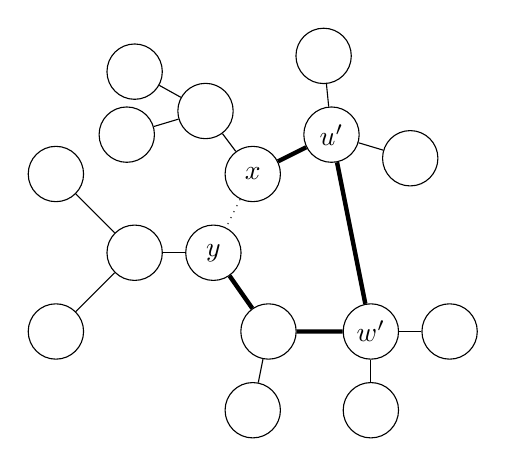
\begin{tikzpicture}
  \node[vertex] (v) at (3, 3.5) {$u'$}; 
  \node[vertex] (c1) at (2, 3) {$x$}; 
  \node[vertex] (c2) at (1.5, 2) {$y$}; 
  \node[vertex] (c3) at (2.2, 1) {}; 
  \node[vertex] (wp) at (3.5, 1) {$w'$}; 
  \node[vertex] (v1) at (2.9, 4.5) {};
  \node[vertex] (v2) at (4, 3.2) {}; 
  \node[vertex] (c11) at (1.4, 3.8) {}; 
  \node[vertex] (c111) at (0.5, 4.3) {}; 
  \node[vertex] (c112) at (0.4, 3.5) {}; 
  \node[vertex] (c21) at (0.5, 2) {}; 
  \node[vertex] (c211) at (-0.5, 3) {}; 
  \node[vertex] (c212) at (-0.5, 1) {}; 
  \node[vertex] (c31) at (2, 0) {}; 
  \node[vertex] (w1) at (4.5, 1) {}; 
  \node[vertex] (w2) at (3.5, 0) {}; 
  % (r) edge[treeEdge, dotted] (u)
  \draw[dotted] (c1) -- (c2); 
  \draw[ultra thick] (c2) -- (c3) -- (wp) -- (v) -- (c1); 
  \draw (v1) -- (v) -- (v2); 
  \draw (c1) -- (c11); 
  \draw (c2) -- (c21); 
  \draw (c3) -- (c31); 
  \draw (c111) -- (c11) -- (c112); 
  \draw (c211) -- (c21) -- (c212); 
  \draw (w1) -- (wp) -- (w2); 
\end{tikzpicture}
\end{center}

As illustrated above,
the observation holds because adding $(u', w')$ to $T^*$ creates a single cycle
(with the path from $u'$ to $w'$ in $T^*$).
Edge $(x, y)$ lies on that cycle, so after removing $(x, y)$ the resulting
set of edges $T'$ is acyclic, and therefore a spanning tree.
(Alternatively, removing $(x, y)$ from $T^*$ disconnects $T^*$
into two disconnected subtrees. One of these contains $u'$, the other contains $w'$.
So adding $(u',w')$ joins the two subtrees into a single spanning tree $T'$.)

Returning to the example, with $(u',w')=(a, c)$,
we can take $(x, y)$ to be any edge on the path from $a$ to $c$ in $T^*$.
That is, one of the edges $(a, d)$, $(d, f)$, or $(f, c)$.
Let's choose $(x, y)$ to be $(a, d)$, the other edge incident to $a$.
Using this edge exchange gives the tree $T'$ shown on the right below:

\begin{center}
\begin{tikzpicture}[scale=0.5]
  \node[vertex] (v) {$a$}; 
  \node [right =of v] {$T^*$ \Large $~\longrightarrow$}; 
  \node[vertex] (w1) [below =of v, xshift=-1.5cm]{$b$}; 
  \node[vertex] (w2) [below =of v, xshift=0cm]{$c$}; 
  \node[vertex] (w3) [below =of v, xshift=1.5cm]{$d$}; 
  \node[vertex] (x1) [below =of w3, xshift=-1.5cm]{$f$}; 

  % (r) edge[treeEdge, dotted] (u)
  \draw (v) -- (w1) node[midway, left] {\footnotesize 3}; 
  \draw[dashed] (v) -- (w2) node[midway, left] {\footnotesize 1}; 
  \draw[ultra thick] (v) -- (w3) node[midway, left] {\footnotesize 1}; 
  \draw (w3) -- (x1) node[midway, left] {\footnotesize 0}; 
  \draw (w2) -- (x1) node[midway, left] {\footnotesize 0}; 
  \draw[dotted] (w1) -- (x1) node[midway, left] {\footnotesize 4}; 
\end{tikzpicture}
\begin{tikzpicture}[scale=0.5]
  \node[vertex] (v) {$a$}; 
  \node [left =of v] {$T'$}; 
  \node[vertex] (w1) [below =of v, xshift=-1.5cm]{$b$}; 
  \node[vertex] (w2) [below =of v, xshift=0cm]{$c$}; 
  \node[vertex] (w3) [below =of v, xshift=1.5cm]{$d$}; 
  \node[vertex] (x1) [below =of w3, xshift=-1.5cm]{$f$}; 

  % (r) edge[treeEdge, dotted] (u)
  \draw (v) -- (w1) node[midway, left] {\footnotesize 3}; 
  \draw[ultra thick] (v) -- (w2) node[midway, left] {\footnotesize 1}; 
  \draw[dashed] (v) -- (w3) node[midway, left] {\footnotesize 1}; 
  \draw (w3) -- (x1) node[midway, left] {\footnotesize 0}; 
  \draw (w2) -- (x1) node[midway, left] {\footnotesize 0}; 
  \draw[dotted] (w1) -- (x1) node[midway, left] {\footnotesize 4}; 
\end{tikzpicture}
\end{center}


% Here's a different way to look at this exchange.
% Recall that a \emph{cut} is a partition $(S,V\setminus S)$
% of the vertices of $G$ into two non-empty sets.
% An edge $(u,w)\in E$
% \emph{crosses} the cut if $u\in S$ and $w\in V\setminus S$.

% \begin{observation}\label{greedy: exchange 2}
%   Let $T$ be any spanning tree of $G$.
%   Let $e$ be any edge in $T$.
%   Consider the cut formed by removing $e$ from $T$.
%   Specifically,  removing $e$ from $T$ splits $T$ into two subtrees $T_1$ and $T_2$,
%   giving the cut  $(S, V\setminus S)$ 
%   where $S$ contains the vertices in $T_1$
%   and $V\setminus S$ contains the vertices in $T_2$.
%   Let $e'$ be any edge crossing this cut.
%   Then removing $e$ from $T$ and adding $e'$
%   gives a spanning tree $T'=\{e'\}\cup T \setminus \{e\}$.
% \end{observation}

% Observation~\ref{greedy: exchange} is equivalent to Observation~\ref{greedy: exchange 2},
% in that $e$ is on the path in $T$ between the endpoints of $e'$
% if and only if $e'$ is on the cut $(S,V\setminus S)$
% defined by removing $e$ from $T$.
% In this note we use only Observation~\ref{greedy: exchange}.
% We use it to show that Rules (i)-(iii) are correct.

Now let's try again to prove the conjecture.
Consider any graph $G$ and edge $(u', w')$, as in the conjecture.
(So $(u',w')$ has minimum weight among edges leaving $u'$.)
Consider any minimum-spanning tree $T^*$ for $G$.
If $(u', w')$ happens to be in $T^*$, then the conjecture holds for $(u', w')$.
But what about the case where $(u', w')$ is not in $T^*$?
Let's try an exchange argument, with a more careful choice of edge to replace.

Let $P$ be the path from $u'$ to $w'$ in $T^*$.
Let $(u', w^*)$ be the edge incident to $u'$ \emph{on this path $P$}.
(In the example, $(u', w^*)$ is $(a, d)$.)
% (Note that $w^* \ne w'$ as $(u', w')$ is not in $T^*$.)
Construct $T'$ from $T^*$ by removing $(u', w^*)$ and replacing it by $(u', w')$,
so $T' = \{(u', w')\} \cup T^* \setminus \{(u', w^*)\}$.
Now, by Observation~\ref{greedy: exchange},
because $(u', w^*)$ is on the path from $u'$ to $w'$ in $T^*$,
\emph{the resulting set $T'$ of edges must be a spanning tree.}

As before, the weight of $(u', w')$ is at most the weight of $(u', w^*)$,
because, among edges leaving $u'$, edge $(u', w')$ (by definition) has minimum weight,
so
\[ \weight {T'} = \weight {T^*} + \weight {u', w'} - \weight {u', w^*} \le \weight{T^*}. \]
Because $T^*$ is an MST, this implies that $T'$ is also an MST.\footnote
{And so, in fact, it must be that $\weight{T'} = \weight{T^*}$, and also $\weight{u', w'} = \weight{u', w^*}$.}
% [review 2026-09-27] fix: conclusion should be that some MST contains the edge $(u', w')$, not "contains $T'$"
And $T'$ does contain $(u', w')$.  Hence, there is an MST that contains $(u', w')$.

So we think we have a line of reasoning by which we know that the conjecture is true.
Here is the conjecture, stated as a lemma,
with a proof that records the details of our reasoning.
\begin{lemma}\label{greedy: lemma: Prim} \PRIMRULE
\end{lemma}
\begin{shortFormProof}
  Let $T^*$ be any minimum spanning tree in $G$.
  If edge $(u', w')$ is in $T^*$, we are done.
  Otherwise, obtain a spanning tree $T'$ from $T^*$ using Observation~\ref{greedy: exchange}
  to add $(u', w')$, selecting the edge $(u', w^*)$ to remove carefully, as follows.
  By definition, the edge $(u', w')$ has minimum weight
  among edges that are incident to $u'$.
  % [review 2026-09-27] fix: the MST in this proof is $T^*$, not $T$
  Let $P$ be the path in $T^*$ connecting $u'$ to $w'$.
  Let $(u', w^*)$ be the edge incident to $u'$ on that path $P$.
  Then take $T' = \{(u', w')\} \cup T^* \setminus \{(u', w^*)\}$.

  By Observation~\ref{greedy: exchange},
  $T'$ is a spanning tree.  
  % [review 2026-09-27] fix: the MST in this proof is $T^*$, not $T$ (two occurrences)
  The weight of $T'$ is at most the weight of $T^*$,
  because $\weight {T'} = \weight {T^*} + \weight {u',w'} - \weight {u', w^*}$,
  and $(u', w')$ has minimum weight among all edges leaving $u'$,
  so $\weight {u', w'} \le \weight {u', w^*}$.
  So $T'$ is also a minimum-weight spanning tree,
  and by construction it contains $(u', w')$.
\end{shortFormProof}

% \begin{lemma}\label{greedy: rule iii}
%   Rule (iii) is correct.
%   That is, given any edge-weighted graph $G=(V,E)$
%   and any edge $e_1$ of $G$ chosen by Rule (iii),
%   there is a minimum spanning tree of $G$ that contains $e_1$.
% \end{lemma}
% \begin{shortFormProof}
%   Let $T$ be any minimum spanning tree in $G$.
%   If $e_1$ is in $T$, we are done.
%   Otherwise, obtain a spanning tree $T'$ from $T$ by using Observation~\ref{greedy: exchange}
%   to add $e_1$, and selecting the edge $e$ to remove as follows.

%   By Rule (iii), the edge $e_1$ crosses some cut $(S,V\setminus S)$
%   and has minimum weight among edges crossing that cut.
%   Let $u'$ and $w'$ be the endpoints of edge $e_1$.
%   Let $P$ be the path between $u'$ and $w'$ in $T$.
%   \emph{Let $e$ be an edge in $P$ that crosses the cut $(S,V\setminus S)$.}
%   (It must exist, as $u'$ is on one side of the cut, and $w'$ is on the other.)

%   Take $T' = \{e_1\} \cup T \setminus \{e\}$.
%   By Observation~\ref{greedy: exchange},
%   $T'$ is a spanning tree containing $e_1$.
%   Then $\weight {T'}$ is at most $\weight T$,
%   because $\weight {T'} = \weight {T} + \weight {e_1} - \weight {e}$,
%   and \emph{$e_1$ has minimum weight among all edges crossing the cut},
%   so $\weight {e_1} \le \weight {e}$.
%   So $T'$ is a minimum-weight spanning tree.
% \end{shortFormProof}

\paragraph{Extending beyond the first edge.}
Fix some input $G=(V,E)$.
The algorithm will start
by choosing some arbitrary vertex $v_0$ in $V$,
and, among edges leaving $v_0$, choosing some edge $(v_0, v_1)$ of minimum weight.
It will choose $(v_0, v_1)$ as its first edge.
By the lemma, this edge is guaranteed to be in some MST.

After committing to connecting $v_0$ and $v_1$ via the edge $(v_0, v_1)$,
one natural way to continue is to choose the cheapest edge leaving the set $\{v_0, v_1\}$.
Then we will have three connected vertices, say $\{v_0, v_1, v_2\}$.
We could then take the cheapest edge leaving those three vertices, and so on.
This idea gives us the following algorithm:

\begin{myframed}
  \begin{steps}
  \item[{{\sf Prim}$(G=(V,E))$:}]
    \comment{--- $G$ is a connected, edge-weighted graph}
    \step choose any vertex $v_0$ in $V$
    \step initialize $T=\emptyset$ and $V_T = \{v_0\}$
    \step for $t=1,2,\ldots,n-1$, where $n=|V|$:
    \begin{block}
      \step among edges leaving $V_T$ (that is, among $\{(u,w)\in E : u\in V_T,\,w\not\in V_T\}$)
      \\\hspace*{3em} let $(u',w')$ be one of minimum weight
      \step add $(u', w')$ to $T$ and add $w'$ to $V_T$
    \end{block}
    \step return $T$
  \end{steps}
\end{myframed}

This is commonly called Prim's algorithm,
although Prim was not the first to discover it.
(See \url{https://en.wikipedia.org/wiki/Prim's_algorithm}.)

\paragraph{Correctness.}
As promised at the start, we'll show that the algorithm maintains the greedy invariant.
For this algorithm, the invariant can be stated specifically as follows:

\medskip 
\centerline{\textsf{greedy invariant}: \emph{the tree $T$ is a subtree of some MST of $G$}}
\medskip 

Lemma~\ref{greedy: lemma: Prim} shows that the invariant holds after the first iteration.
By using more or less the same reasoning, we show that every iteration maintains the invariant.

\begin{lemma}\label{greedy: invariant}
  Throughout any execution of the algorithm, the invariant holds.
\end{lemma}
\begin{longFormProof}
  \step Consider any execution of the algorithm on some connected graph $G=(V,E)$.
  \step At the start of the first iteration, $T$ is a singleton vertex.
  \step Since $G$ is connected, it has some MST, so the invariant holds initially.
  \step Next we show that each iteration maintains the invariant.
  \begin{block}[greedy: iter]
    \step Consider any iteration such that the invariant holds at the start of the iteration.
    \step Let $T$ be the subtree just before the iteration.  
    \step Let $(u',w')$ be the edge chosen in the iteration.
    \step[greedy: rule] So $(u', w')$ leaves $V_T$,
    and has minimum weight among edges leaving $V_T$.
    \step The invariant holds at the start of the iteration, so $T$ is a subtree of some MST, say $T^*$.
    \begin{block}[greedy: C1]
      \step \underline{Case 1.}  Suppose $T^*$ contains $(u', w')$ as well.
      \step Then $T\cup\{(u',w')\}$ is also a subtree of $T^*$, so the invariant holds at the end of the iteration.
    \end{block}
    \begin{block}[greedy: C2]
      \step \underline{Case 2.}  Otherwise $(u', w')$ is not in $T^*$.
      \step The edge $(u', w')$ leaves $V_T$,
      so at least one edge on the path in $T^*$ from $u'$ to $w'$ leaves $V_T$.
      \step Let $(x, y)$ be such an edge.
      % \step So $(u', w')$ is not in $T^*$, and $(x,y)$ is on the path in $T^*$ between $u'$ and $w'$.
      \step By Observation~\ref{greedy: exchange}, adding $(u', w')$ to $T^*$
      and removing $(x, y)$ gives the spanning tree $T'$ where
      \[T' = \{(u', w')\} \cup T^* \setminus \{(x, y)\}.\]
      \step Edge $(x,y)$ leaves $V_T$, while edge $(u', w')$ has minimum weight among edges leaving $V_T$.
      \step So $\weight{u', w'} \le \weight {x, y}$.
      This implies that $\weight{T'} = \weight{T^*} +\weight{u', w'} - \weight {x, y} \le \weight{T^*}$.
      \step So $T'$ is also a minimum-weight spanning tree of $G$.
      \step Edge $(x, y)$ leaves $V_T$, so $(x, y)$ is not in $T$.
      \step So, at the end of the iteration,
      the new subtree $T\cup \{(u', w')\}$ is a subtree of MST $T'$.
      \step So the invariant holds at the end of the iteration.
    \end{block}
    \step By Cases 1 and 2 above, the invariant holds at the end of the iteration.
  \end{block}
  \step As observed previously, the invariant holds at the start of the first iteration.
  \step By Block~\ref{greedy: iter}, each iteration maintains the invariant.  So it holds throughout.
\end{longFormProof}

Correctness of the algorithm follows easily from the invariant:

\begin{theorem}
  Prim's algorithm is correct.
  Given any connected edge-weighted graph $G$,
  it returns a minimum spanning tree for $G$.
\end{theorem}
\begin{shortFormProof}
  Consider any execution of the algorithm on any input $G$.
  By Lemma~\ref{greedy: invariant}, the invariant holds after the last
  iteration of the algorithm, so the final subtree $T$
  is a subtree of some minimum spanning tree $T^*$ of $G$.
  Since each of the $n-1$ iterations adds a new vertex to $T$,
  at termination $T$ contains all $n$ vertices,
  so $T$ is itself a spanning tree of $G$.
  So $T=T^*$.  That is, $T$ is a minimum spanning tree.
\end{shortFormProof}


\paragraph{Run time.}
For efficiency, % (just as in Dijkstra's algorithm),
the algorithm can maintain the edges $(u,w)$ leaving $V_T$ in a heap,
keyed by $\weight {u, w}$.
Then choosing the best edge $(u', w')$ in each iteration takes $O(\log n)$ time.
The algorithm maintains the heap when $w'$ is added to $V_T$ as follows.
For each edge $(w', x)$ incident to $w'$,
if $x$ is in $V_T$, then it removes $(w', x)$ from the heap,
and otherwise ($x$ is not in $V_T$) it adds $(w', x)$ to the heap.
The time for the iteration is then $O((1+\textsf{degree}(w')) \log n)$,
so the total time is $O(\log n \sum_{w'\in V} 1 + \textsf{degree}(w')) = O((n+m)\log n)$:

We have the following result:
\begin{theorem}
  There is an $O((m+n)\log n)$-time algorithm for the \prob{Minimum Spanning Tree} problem.
\end{theorem}

This algorithm is similar to Dijkstra's shortest-path algorithm.\footnote
{In each iteration,
the algorithm chooses, among edges $(u, w)$ leaving $V_T$, one that minimizes $\weight {u, w}$,
whereas Dijkstra's algorithm chooses,
among edges $(u, w)$ leaving $K$, one that minimizes $d[u] + \weight {u, w}$.}

\pythonCode{greedy_algorithms/min_spanning_tree.py}

\subsection{A recursive view}
Many greedy algorithms make one greedy choice, then recurse.
Unwinding the tail recursion gives an iterative algorithm.
Next we describe how Prim's algorithm (and others)
can be developed via this recursive approach,
instead of by the iterative view in the previous section.

Recall the first greedy step:
choose any vertex $u'$
and an edge $(u', w')$ of minimum weight among edges leaving $u'$,
then commit to taking edge $(u', w')$.
By Lemma~\ref{greedy: lemma: Prim}, this edge is in some MST.

To continue, don't proceed iteratively as in the previous section.
Instead, imagine \emph{contracting} the edge $(u', w')$ into a single vertex.
Contraction replaces $u'$ and $w'$ in the graph
by a single new vertex, say $v'$,
which inherits all of the edges incident to $u'$ or $w'$
(except for the edge $(u', w')$, which is deleted).
Let $G'$ be the graph obtained from $G$ by contracting $(u', w')$.

With some thought, one can show,
for any set $R$ of edges (except $(u',w')$) 
that $\{(u', w')\} \cup R$ is a spanning tree of $G$
if and only if $R$ is a spanning tree of $G'$.
Using this and an easy edge-weight calculation, one can prove this observation:
\begin{observation}\label{greedy: contraction}
  Let $R$ be any MST of $G'$.
  Then $\{(u', w')\} \cup R$ is an MST of $G$.
\end{observation}

Hence, to find a set $R$ of edges such that $\{(u', w')\} \cup R$ is an MST,
it suffices to compute an MST in $G'$, and take $R$ to be that one.
This gives the following recursive algorithm:
\begin{myframed}
  \begin{steps}
  \item[{{\sf rGreedyMST}$(G=(V,E))$:}]
    \comment{--- $G$ is a connected, edge-weighted graph}
    \step if $|V|=1$: return $\emptyset$
    \step choose any vertex $u'$ in $V$
    \step among edges leaving $u'$, let $(u', w')$ be one of minimum weight
    \step let $G'$ be the graph obtained from $G$ by contracting $(u', w')$
    \step $R \gets \textsf{rGreedyMST}(G')$
    \step return $\{(u', w')\} \cup R$
  \end{steps}
\end{myframed}

This algorithm is correct by induction,
using Observation~\ref{greedy: contraction} to show the inductive step.
(By induction, $R$ is an MST of $G'$,
so by the observation $\{(u', w')\} \cup R$ is an MST of $G$.)

Prim's algorithm can viewed as the above algorithm,
where in each recursive call the vertex $u'$ is taken
to be the new vertex that was just formed by the edge contraction in the parent call.
This way, as the algorithm proceeds, the edges contracted so
far form just one connected subtree in the original graph.
This is the subtree $T$ in the iterative version of Prim's algorithm.
  
% \subsection*{Other greedy MST algorithms}

\paragraph{Kruskal's algorithm.}
We can obtain other greedy MST algorithms
by choosing the vertex $u'$ in other particular ways in each call.
Consider the following rule:
\emph{let $(u', w')$ be any edge of minimum weight in the entire graph}.
(We can have the algorithm choose this $u'$ in Step 2,
and, in Step 3, have it take edge $(u', w')$ out of $u'$.
This edge is guaranteed to be a minimum-weight edge out of $u'$,
so it is a correct choice for the algorithm.)
So the the following recursive algorithm is also correct:
\begin{myframed}
  \begin{steps}
  \item[{{\sf rGreedy2}$(G=(V,E))$:}]
    \comment{--- $G$ is a connected, edge-weighted graph}
    \step if $|V|=1$: return $\emptyset$
    \step let $(u', w')$ be a minimum-weight edge in $G$
    \step let $G'$ be the graph obtained from $G$ by contracting $(u', w')$
    \step $R \gets \textsf{rGreedy2}(G')$
    \step return $\{(u', w')\} \cup R$
  \end{steps}
\end{myframed}

Next we unwind the tail recursion in this algorithm,
and, instead of contracting each chosen edge, 
we just maintain the set $F$ of edges that have been chosen so far.
(As the algorithm proceeds,
$F$ will form a forest --- a collection of disjoint subtrees.
If we were to contract the edges in $F$,
each subtree would contract to a vertex
giving us back the contracted graph in the algorithm above.)
This yields the following iterative algorithm:
\begin{myframed}
  \begin{steps}
  \item[{{\sf iGreedy2}$(G=(V,E))$:}]
    \step initialize  $F$ to be the forest with vertex set $V$ and no edges.  let $n=|V|$.
    \step for $t=1,2,\ldots,n-1$:
    \begin{block}
      \step among edges connecting any two subtrees in $F$, let $(u', w')$ be one of minimum weight 
      \step add $(u', w')$ to $F$ (joining the two trees into one)
    \end{block}
    \step return $F$
  \end{steps}
\end{myframed}

Each iteration adds a minimum-weight edge among edges connecting different subtrees,
so we can also implement this algorithm as follows:

\begin{myframed}
  \begin{steps}
  \item[{{\sf Kruskal}$(G=(V,E))$:}]
    \comment{\normalsize --- Kruskal's algorithm ---}
    \step initialize  $F$ to be the forest with vertex set $V$ and no edges.  let $n=|V|$.
    \step let $e_1, e_2, \ldots, e_m$ be the edges in $E$, ordered by increasing weight
    \step for $t=1$ to $m$:
    \step~~~if $e_t$ connects different subtrees in $F$: add $e_t$ to $F$
      \comment{but how do we check this?}
    \step return $F$
  \end{steps}
\end{myframed}

This is known as Kruskal's algorithm.
We haven't specified how to determine whether $e_t$ connects different subtrees in $F$.
One naive way is to use depth-first search in $F$,
but that takes linear time, leading to a quadratic-time algorithm.
A better way uses a \emph{disjoint-set} data structure.
We haven't studied it, but, using that data structure,
the total time will be dominated by the time to sort the edges.
So the total time will be $O((m+n)\log n)$, where $m=|E|$ and $n=|V|$.

% \paragraph{Generic algorithm.}
% If we allow the full generality of Rule (iii),
% we get the following generic algorithm.
% It generalizes both Prim's algorithm and Kruskal's algorithm.
% As the algorithm proceeds,
% it applies Rule (iii) to the graph
% obtained by contracting all edges in $F$.
% (In the contracted graph, each vertex corresponds to a subtree of $F$.)

% To define the algorithm,
% say that a cut $(S, V\setminus S)$ \emph{respects} $F$
% if none of the edges in $F$ cross the cut.
% Equivalently, each subtree in $F$ is either entirely within $S$,
% or entirely within $V\setminus S$.

% \begin{myframed}
%   \begin{steps}
%   \item[{{\sf gMST}$(G=(V,E))$:}]
%     \comment{\normalsize --- generic MST algorithm ---}
%     \step initialize $F \leftarrow \emptyset$
%     \step while there exists a cut that respects $F$ (i.e., no edges in $F$ cross the cut):
%     \begin{block}
%       \step choose any cut $(S, V\setminus S)$ that respects $F$
%       \step let $e_t$ be any edge having minimum weight among edges crossing the cut

%       (at least one edge crosses the cut, as $G$ is connected) 

%       \step add $e_t$ to $F$
%     \end{block}
%     \step return $F$
%   \end{steps}
% \end{myframed}

% For completeness, here is a proof that the generic algorithm is correct.

% \begin{lemma}\label{greedy: invariant}
%   The generic algorithm maintains the following invariant:
%   the current set $F$ of edges is contained in some minimum spanning tree.
% \end{lemma}
% \begin{longFormProof}
%   \step Consider any execution of the algorithm on some input $G=(V,E)$.
%   \step The invariant holds before the first iteration, when $F=\emptyset$.
%   \begin{block}[greedy: iter]
%     \step Consider any iteration $t$ such that the invariant holds before the iteration.
%     \step Let $F$ denote $F$ at the start of the iteration.
%     \step Let cut $(S, V\setminus S)$ and $e_t=(u,w)$ be as chosen in the iteration.
%     \step[greedy: rule] So the cut respects $F$,
%     and $e_t$ has minimum weight among edges crossing the cut.
%     \step Let $T$ be a minimum spanning tree such that $F\subseteq T$
%     (per the invariant).
%     \begin{block}[greedy: C1]
%       \step \underline{Case 1.}
%       First consider the case that $e_t \in  T$.
%       \step Then $F\cup\{e_t\} \subseteq T$,
%       so the invariant holds at the end of the iteration.
%     \end{block}
%     \begin{block}[greedy: C2]
%       \step \underline{Case 2.}  Otherwise $e_t\not\in T$.
%       \step The edge $e_t$ crosses the cut,
%       so the path in $T$ between $e_t$'s endpoints crosses the cut.
%       \step So some edge on that path crosses the cut. Let $e$ be such an edge.
%       \step So $e_t$ is not in $T$, and $e$ is on the path in $T$ between the endpoints
%       of $e_t$.
%       \step By Observation~\ref{greedy: exchange}, adding $e_t$ to $T$
%       and removing $e$ gives a spanning tree $T' = \{e_t\} \cup T \setminus \{e\}$.
%       \step Edge $e_t$ has minimum weight among edges crossing the cut
%       (including $e$) so $\weight{e_t} \le \weight e$.
%       \step So $\weight{T'} = \weight{T} +\weight{e_t} - \weight e \le \weight{T}$.
%       \step So $T'$ is also a minimum-weight spanning tree of $G$.
%       \step Edge $e$ crosses the cut, and the cut respects $F$, so $e\not\in F$.
%       \step So $\{e_t\}\cup F \subseteq \{e_t\}\cup T \setminus\{e\} = T'$.
%       \step So, at the end of the iteration,
%       the partial solution $F\cup\{e_t\}$ is a subset of the MST $T'$.
%       \step So the invariant holds at the end of the iteration.
%     \end{block}
%     \step By Blocks~\ref{greedy: C1} and~\ref{greedy: C2},
%     the invariant holds at the end of the iteration.
%   \end{block}
%   \step By Block~\ref{greedy: iter}, each iteration that starts with the invariant true ends with it true.
%   \step And, as observed above, the invariant holds initially.  So it holds throughout.
% \end{longFormProof}

% \begin{theorem}
%   The generic algorithm is correct.
%   Given any connected edge-weighted graph $G$,
%   it returns a minimum spanning tree for $G$.
% \end{theorem}
% \begin{shortFormProof}
%   Consider any execution of the algorithm on any input $G$.
%   By Lemma~\ref{greedy: invariant}, the invariant holds after the last
%   iteration of the algorithm, so the final set $F$
%   is a subset of some minimum spanning tree $T$ of $G$.
%   By the termination condition of the loop,
%   $F$ must connect all vertices in $G$
%   (otherwise some cut would respect $F$).
%   There cannot be any edge in $(u,w)\in T\setminus F$
%   (otherwise $(u,w)$ and the path in $F$ from $u$ to $w$
%   would form a cycle in $T$,
%   contradicting that $T$ is a tree).
%   So $F=T$.  That is, $F$ is a minimum spanning tree.
% \end{shortFormProof}

\pythonCode{greedy_algorithms/min_spanning_tree.py}

\subsection{Exercises}

\paragraph{External exercise with solutions}
\begin{itemize}
\item \KT Solved Exercises 3 (MSTs)
\end{itemize}

\paragraph{Exercises without solutions}

\exercise \emph{(Simulate Prim)} % CS 3000 F18 HWK 7 Problem 4
Manually simulate Prim's algorithm (from the lecture notes) on the graph $G$ below, starting from source $s$.
List the edges that the algorithm chooses, in the order that it chooses them.

\begin{center}
  \begin{tikzpicture}[
    vertex/.style={circle, inner sep=0pt, minimum width=15pt, draw},
    every path/.style={}
    ]
    \node[vertex] (s) {s}; 
    \node[vertex] (a) [right =of s, xshift=-15pt, yshift=30pt] {a}; 
    \node[vertex] (b) [right =of a] {b}; 
    \node[vertex] (c) [right =of b] {c}; 
    \node[vertex] (d) [right =of s, xshift=-15pt, yshift=-30pt] {d}; 
    \node[vertex] (f) [right =of d] {f}; 
    \node[vertex] (g) [right =of f] {g}; 
    \node[vertex] (x) [right =of s, xshift=7pt] {x}; 
    \node[vertex] (y) [right =of x, xshift=45pt] {y}; 

    \path (s) edge node [midway, auto] {4} (a); 
    \path (s) edge node [pos=0.3, below] { 9}  (d);
    \path (a) edge node [midway, left] { 11}  (d);
    \path (a) edge node [midway, auto] { 8}  (b);
    \path (b) edge node [midway, auto] { 7}  (c);
    \path (d) edge node [midway, below] { 1}  (f);
    \path (f) edge node [midway, below] { 2}  (g);
    \path (d) edge node [pos=0.8, below] { 7}  (x);
    \path (x) edge node [pos=0.7, left] { 2}  (b);
    \path (b) edge node [midway, left] { 4}  (g);
    \path (x) edge node [pos=0.6, left] { 6}  (f);
    \path (c) edge node [pos=0.3, left] { 14}  (g);
    \path (g) edge node [pos=0.7, below] { 10}  (y);
    \path (c) edge node [pos=0.7, above] { 9}  (y);
  \end{tikzpicture}
\end{center}




\exercise\emph{(MST proof check)}
\begin{conjecture}
  Let $G$ be any connected edge-weighted graph $G$ with at least two vertices.
  Let $v$ be any vertex,
  and, among edges leaving $v$,
  let $(v, w^*)$ be one of minimum weight.
  Suppose every other edge incident to $v$ has larger weight.
  Then $(v,w^*)$ is in \emph{every} minimum spanning tree of $G$.
\end{conjecture}
\begin{longFormProof}
  \step Consider any such graph $G$, vertex $v$, and edge $(v,w^*)$,
  \begin{block}[greedy: T]
    \step Consider any spanning tree $T$ of $G$ that does not contain $(v,w^*)$.
    \step Since $T$ is connected and contains all vertices, $T$ contains some edge incident to $v$.
    \step Let $(v, w')$ be such an edge.  Note that $w' \ne w^*$ as $(v, w^*)$ is not in $T$.
    \step Let $T' = \{(v, w^*)\} \cup T \setminus \{(v, w')\}$ be obtained from $T$ by removing $(v, w')$ and adding $(v, w^*)$.
    \step Then $\weight{v, w^*}$ is strictly less than $\weight{v, w'}$.  That is, $\weight{v, w^*} < \weight{v, w'}$.  
    \step So $\weight{T'} = \weight{T} + \weight{v, w^*} - \weight{v, w'} < \weight T$.
    \step So $T'$ is a spanning tree whose total weight is strictly less than the total weight of $T$.
    \step So $T$ is not a minimum spanning tree.
  \end{block}
  \step By Block~\ref{greedy: T}, every spanning tree of $G$ that doesn't contain $(v, w^*)$ isn't a minimum spanning tree. 
  \step So every minimum spanning tree of $G$ contains $(v, w^*)$.
\end{longFormProof}

Is the reasoning in the proof correct?
If not, what is the first step that makes an assertion that is not necessarily true,
given the assumptions?
Why exactly is that assertion not necessarily true?

\exercise\emph{(Reverse greedy MST)}
Here's another kind of greedy algorithm to consider.
Start with all edges in the graph,
and \emph{remove} edges one by one,
until the remaining edges form a spanning tree.
Can you come up with an algorithm of this form?

\begin{enumerate}[label=(\alph*)]
\item Define an iterative MST algorithm based on the following rule:

  \emph{Let $C$ be any cycle in the remaining graph,
    and remove any maximum-weight edge on $C$.}

\item Prove that the rule maintains this invariant: 

  \emph{Some minimum spanning tree of the original graph
    is a subset of the remaining edges}.

\item  Prove that the algorithm is correct (use that it maintains the invariant).
\end{enumerate}
As much as possible, follow the structure of the proofs in Section~\ref{greedy: sec: prims}.


\paragraph{External exercises without solutions}
\begin{itemize}
\item \JE Chapter 7, Exercises 1--10 
\item \DPV Exercises  5.1--5.10, 5.21--5.23
\item \KT Chapter 4, Exercises 1--3, 8--11, 19--23, 27, 28, 31
\item \CLRS Exercises in Chapter 23
\end{itemize}


\subsection{External sources on \prob{Minimum Spanning Tree}}

\begin{itemize}

\item \DPV Section 5.1;
  \KT Section 4.5 and \KWSlides;
  \CLRS Chapter 23;
  \JE Chapter 7

\item MIT lecture video: 

  \parbox{5in}{  
\url{https://ocw.mit.edu/courses/electrical-engineering-and-computer-science/6-046j-introduction-to-algorithms-sma-5503-fall-2005/video-lectures/lecture-16-greedy-algorithms-minimum-spanning-trees/}}

\end{itemize}


%%% Local Variables:
%%% mode: latex
%%% TeX-master: "greedy_algorithms"
%%% End:
